\documentclass[columns=,boxcolor=white]{datart}

%\usepackage[top=1in,bottom=1in,left=1.2in,right=1.2in]{geometry}

%\usepackage{stmaryrd} % For those delicious brackets

% Title
\title{Big Data Problem with Machine Intelligence Stuff}
\date{}

\author[1]{Anders Roland Nielsen}
\author[1]{Andreas Berre Eriksen}
\author[1]{Kent Munthe Caspersen}
\author[1]{Mathias Melgaard Andersen}
\author[1]{Mikkel Alexander Madsen}
\author[1]{Sander Jespersen}

\affil[1]{Department of Computer Science, Aalborg University}

% CLEVEREF
%\crefname{tempDef}{Definition}{Definitions}
%\crefname{tempProof}{Proof}{Proofs}

%COMMANDS
%\usepackage{lmodern}

%HÜTTEL RULES
\providecommand{\condinfrule}[3]{\parbox{5.5cm}{\[ {\frac{#1}{#2}}{\qquad #3} \hfill \]}}
\providecommand{\infrule}[2]{\parbox{4.5cm}{\[\frac{#1}{#2}\hspace{.5cm}\]}}
\providecommand{\runa}[1]{\ensuremath{\tt{[#1]}}}
\providecommand{\single}[1]{\ensuremath{#1} \\}
\providecommand{\singlemat}[1]{\parbox{4.5cm}{\[#1\hspace{.5cm}\]}}
\providecommand{\bigrule}[2]{\genfrac{}{}{0pt}{0}{#1}{#2}}

% Gordon
% ----------------------------------------------------------------- %
% Horizontal brackets.                                              %
% ----------------------------------------------------------------- %

\newcommand{\hbra}{
%\hbox to .995       \columnwidth{\vrule width0.3mm height 1.8mm depth-0.3mm
\hbox to .995       \linewidth{\vrule width0.3mm height 1.8mm depth-0.3mm
                    \leaders\hrule height1.8mm depth-1.5mm\hfill
                    \vrule width0.3mm height 1.8mm depth-0.3mm}}
\newcommand{\hket}{
\hbox to .995 
%                    \columnwidth{\vrule width0.3mm height1.5mm
                    \linewidth{\vrule width0.3mm height1.5mm
                    \leaders\hrule height0.3mm\hfill
                    \vrule width0.3mm height1.5mm}}

% ----------------------------------------------------------------- %
% Typesetting definitions:                     output:              %
%                                                                   %
% \begin{defn}                                                      % 
% \Category{M,N}{terms}\\               M, N ::=      terms         %
% \entry{x}{variable}\\                   x             variable    % 
% \entry{M\ N}{application}\\             M N           application %
% \entry{\lambda x.\ M}{abstraction}      \x.M          abstraction %
% \end{defn}                                                        %
%                                                                   %
% This is a tabbing environment; the last entry should have no \\.  %
% ----------------------------------------------------------------- %

\makeatletter
  \newcommand{\addToLabel}[1]{%
    \protected@edef\@currentlabel{\@currentlabel#1}%
  }
\makeatother

\newcommand{\ratio}{.3}

\newenvironment{display}[1]{
  \pagebreak[2]% to prevent ugly broken displays
\begin{tabbing}
%\hspace{1.5em} \= \hspace{\ratio\columnwidth-1.5em} \= \hspace{1.5em} \= \hspace{1.5em} \= \kill
\hspace{1.5em} \= \hspace{\ratio\linewidth-1.5em} \= \hspace{1.5em} \= \hspace{1.5em} \= \kill
  {\bfseries#1}\\[-.7ex]
  \hbra\\[-.6ex]
  }{\\[-.7ex]\hket
  \end{tabbing}\vspace{-1.0ex}\normalsize}

\newcommand{\entry}[2]{\>$#1$\>\>#2}
\newcommand{\clause}[2]{$#1$\>\>#2}
\newcommand{\Category}[2]{\clause{#1::=}{#2}}
\newcommand{\simplecategory}[3]{\clause{#1::=#2}{#3}}
\newcommand{\subclause}[1]{\>\>\>#1}
\newcommand{\redrule}[3]{$#1$\>\>$#2$\>\>\>#3}

\newcommand{\labelledClause}[2]{%
  $#1$
  \>\>\>{\small #2}%
  \refstepcounter{rule}%
  \addToLabel{#2}%
}

\newcommand{\wlabelledClause}[2]{%
  $#1$
  \>\>\>\>{\small #2}%
  \refstepcounter{rule}%
  \addToLabel{#2}%
}


% \newcommand{\nodisplaybreak}[1]{ 
%   \noindent\begin{minipage}{\columnwidth}#1
%   \end{minipage}}

% \newcommand{\nofulldisplaybreak}[1]{ 
%   \iffull\begin{tabbing}\nodisplaybreak{#1}\end{tabbing}\else{#1}\fi}  \hbra\\[-.6ex]
%   }{\\[-.7ex]\hket
%   \end{tabbing}\vspace{-1.0ex}\normalsize}

% \newcommand{\entry}[2]{\>$#1$\>\>#2}
% \newcommand{\clause}[2]{$#1$\>\>#2}
% \newcommand{\Category}[2]{\clause{#1::=}{#2}}
% \newcommand{\simplecategory}[3]{\clause{#1::=#2}{#3}}
% \newcommand{\subclause}[1]{\>\>\>#1}
% \newcommand{\redrule}[3]{$#1$\>\>$#2$\>\>\>#3}




% document
\begin{document}
\usetikzlibrary{arrows,intersections,shapes.geometric,calc}
\maketitle

% ABSTRACT
\begin{abstract}
Here be dragons.
\end{abstract}

%%% Local Variables:
%%% mode: latex
%%% TeX-master: "main"
%%% End:


% CONTENT
\section{Introduction}\label{sec:intro}

Online multiplayer games have the possibility of generating a lot of data, this increases with the possible options for each individual player and the number of players. 
League of Legends (LoL), created by Riot games, was the most played online game in the beginning of 2015~\cite{LoLmostplayed}, mustering 27 million people playing it daily in the beginning of 2014~\cite{LoL27mill}. 

When playing, the players are divided into 2 competing teams (blue, purple) of 5 players each. In a classic match, each player will pick a champion(character) from a pool of 124 champions, each champion with 4 unique abilities. An ability is a magic spell, which does wildly different things, such as throwing a fireball at an opponent.
\\

\begin{wrapfigure}{r}{{0.5\textwidth}}
  \centering
    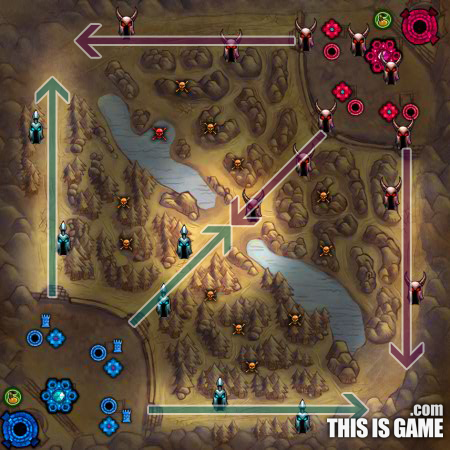
\includegraphics[width=0.5\textwidth]{Section1/lolmap.png}
  \caption{League of legends map}
\end{wrapfigure}\label{lolmap}
The map consists of three lanes(top, middle, bottom) as shown with arrows, connecting the two bases. In front of each lane in each base are two structures, an inhibitor and a turret defending the inhibtor. In the middle of the base is the nexus, which when destroyed ends the game, making the enemy team the winner. In each lane, the inhibitors spawn creeps(small monsters with low damage and health) which walks toward the opposing base on the lane it was spawned, the effect is that the two team's monsters meet in the middle, which is where the teams will fight, killing each others creeps. Furthermore, each lane has two extra turrets outside the base. A turret is a defensive structure fires at approaching enemies. When the inhibitor is destroyed, it makes the opposing team summon stronger minions. Lastly note that there is a "jungle", which consists of stronger monsters which award gold, and experience.
\\
Experience and money is earned through out the game for the individual players, when killing monsters or opposing players. The experience is used to improve the skills of the champion while money is spend purchasing items that will make the player stronger. This sums up the most important aspects of the game, and it is already quite clear how statespace the game hosts. This makes it extremely complex, and very interesting to analyse what one can do to improve ones gameplay. 
\\\\
The game combines strategy, individual player skill, communication and team play. It is a massive skill showcase, but how important is strategy? In this paper we will investigate how much of an advantage one can get by making good strategic decisions, based on a large dataset of matches played.


\subsection{Related Work}\label{sec:relatedwork}
K.\ Conley and D.\ Perry have trained a classifier to predict the winning team of a Dota 2 match~\cite{dota2article}, by only considering the heroes chosen at the beginning of the game. Dota 2 is game very similar to LOL.\@
Each feature used, represents the presence or absence of a particular hero on one of the teams.
When training on 18,000 matches they could correctly predict the outcome of 69.8 \% of the 5,669 matches in their test set.
With 50,000 training samples, they almost reached 70 \% correct predictions. Only matches between players of similiar skill levels were considered.

Konstantin Shvachko, et al.\, created Hadoop distributed file system (HDFS), to reliably handle very large data and to stream that data to user application at high bandwidth. They described the architecture and showed that it can successfully handle 25PB of Yahoo enterprice data~\cite{HDFS}.

Hadoop MapReduce and different variants have successfully been used for big data problems, by distributing the work load between many nodes in a cluster~\cite{DeanMapReduce}. 
Matei Zaharia, et al.\ have created Apache Spark and using this framework, the computation time is reduced if the data is being reused, in e.g.\ iterative machine learning or iterative data analysis tools~\cite{ApacheSpark}. 



%%% Local Variables:
%%% mode: latex
%%% TeX-master: "../main"
%%% End:

\section{Preliminaries}\label{sec:prelim}
\subsection{Big Data Problem}
A problem can be described as a big data problem if the problem is thoroughly complex, such that conventional data processing cannot be applied. There is no direct line definition of when something is complex is enough, it is up to the individual solving the problem, if one wishes to apply big data techniques to solve it. However, there are three main variables which contribute to the complexity, namely: Volume, velocity, variety. Volume is the amount of storage the data occupies, velocity is identified as the rate at which the data grows and lastly variety is seen as the complexity or how much it varies of the data. 
Every problem is thus a combination of these three variables. One might naively think that big data problems are not that different from any other problem, ``just more data!''. The problem which we are concerned with in this project, it is mostly the volume which is large. 

In big data problems traditional data processing tools do not scale well. Instead one usually distributes the data across multiple machines using various distributed systems. It is important to recognize that solving a big data problem, introduces new challenges both in terms of storage and complexity. This means that certain machine learning algorithms are more applicable, since the problem will have to be split up and computed in parallel.  We will briefly look at one technique for solving big data problems in the next section.
%http://www.computer.org/csdl/mags/ic/2012/03/mic2012030004.pdf    %From Databases to Big Data

\subsubsection{MapReduce} % (fold)
\label{sec:mapreduce_programming_model}

MapReduce is a programming model which is especially used in the context of ``Big Data''. The model is useful in the context of processing large amounts of data, utilizing parallelization. The main reason for the success of the MapReduce model, is mostly because it is easy for the programmer to parallelize, and its low-cost, high-compute property. MapReduce is well-suited in a distributed computing setting, handling data large enough to not fit into a single disk.

MapReduce is comprised of a \emph{map} procedure and a \emph{reduce} procedure, which is where the name comes from. The two procedures are split into the following actions:


\begin{description}
    \item[Map] This procedure takes as input a key-value pair and ``sets-up'' the data, by e.g. filtering or sorting. The resulting output is an intermediate key-value pair used for input to the reduce function.
    \item[Reduce] This procedure takes an intermediate key and a set of values for that key, it then reduces by merging these values into a result
\end{description}
%src: http://static.googleusercontent.com/media/research.google.com/da//archive/mapreduce-osdi04.pdf

\subsubsection{Complications of distributed computing}

Outline of this section:
- Similarity with parallel programming
    - Shared memory vs. network message passing
- Pre-compute feature name/index map
- Transforming/referencing RDD can only happen one at a time
- HDFS data is immutable
- 






\subsection{Logistic Regression}\label{sec:logistic}

To predict the outcome of a match, we use a linear classification model.
The model consists of a hypothesis function that is linear in the parameters.

\[ \hat{y} = w_0 + \sum_{j=1}^{M-1} w_j \phi_j(x) \]

Where $w_j$ represents the impact of of $\phi_j(x)$ on the hypothesis,
$w_0$ is the intercept and $\phi_j$ is a basis function that
performs a transformation on the input features. 

In order to classify the result of the hypothesis function into wins and losses. 
We use the so called logistic or sigmoid function.

\[ \sigma(\textbf{x}) = \frac{1}{1+e^{- \textbf{x}}} \]

The sigmoid function squashes the result of the hypothesis function into an inverval between one and zero.
This is appropriate because we never want a prediction less than zero or greater than one on a binary feature.
Furthermore the sigmoid function has a simple derivative that makes it easy to work with when using iterative methods.

\[ \sigma'(x) = \sigma(x) \times (1-\sigma(x)) \] 

\subsubsection{Cost Function}

In order to find the weights that produce the most accurate classification.
We minimise the squared error function.

\[ E_D = \sum_{n=1}^{N} \left(y_n - \textbf{w} \phi(\textbf{x}_n) \right)^2 \] 

\subsubsection{Regularisation}
To combat the problem of overfitting, we can use a method called L2-Regularisation.
In regularisation we penalise large weights, by adding the following term to the cost function.

\[ E_w = \lambda \sum_{j=1}^{M-1} w_j^2 \]

Where the regularisation constant $\lambda$ scales the penalty. 
The new cost function looks like this.

\[ E(\textbf{w})
  = E_D + E_w 
  = \sum_{n=1}^{N} \left(y_n - \textbf{w} \phi(\textbf{x}_n) \right)^2 + \lambda \sum_{j=1}^{M-1} w_j^2 \]

\begin{flushright}
\cite[online course]{courseraAI}
\end{flushright}

\subsubsection{Batch Gradient Descent}

Since we are using a large number of features, applying an analytic solution to find the weights quickly becomes impractical.
Therefore we use an iterative approach called batch gradient descent.

In gradient descent we iteratively update the weights by the partial derivative of the cost function with respect to the weight, multiplied by a learning rate $\eta$  
\[ w_j \leftarrow w_j - \eta \nabla_w E(\textbf{w}) \]

\subsubsection{Stochastic Gradient Descent}\label{sec:stochastic}

%When dealing with large data sets calculating the sum in the cost function becomes problematic.
 


% Non convergence of stochastic gradient descent





\begin{flushright}
\cite{Bishop2006}[p. ??]
\end{flushright}

% ###################################################################
%
%%\subsection{Logistic Regression}\label{sec:logistic}
%\subsection{Logistic Regression (old)}
%% logistic function
%
%For classification we use an activation function, whose purpose is to squash the result into the interval $(0,1)$.
%\[ f^{\overline{w}}(X_1, X_2, \dots X_n) = f(w_0 + w_1 \times X_1 + w_2 \times X_2 + \cdots + w_n \times X_n) \]
%
%\paragraph{Activation Functions}
%
%The most basic activation function is the so called step function defined as 
%\[ f(x) = \begin{cases}
%%	1 &\text{ if } f^{\overline{w}}(X_1,X_2, \text{ ... }, X_n) > 0 \\
%%	0 &\text{ if } f^{\overline{w}}(X_1,X_2, \text{ ... }, X_n) \leq 0 
%
%	1 &\text{ if } x \geq 0 \\
%	0 &\text{ if } x < 0 
%\end{cases}\]
%
%However the step function is not differentiable, and since this is a requirement for gradient descent we use another
%function called the sigmoid or logistic function.
%\[ f(x) = \frac{1}{1+e^{-x}} \]
%Unlike the previous activation function this function has a very simple derivative.
%
%\[ f'(x) = f(x) \times (1-f(x)) \]
%
%Which makes it easy to implement in a gradient descent algorithm.
%
%The cost function then becomes.
%\[ Error_E(\overline{w}) = \sum_{e \in E} \left(val(e,Y)-f\left(pval^{\overline{w}}(e,Y)\right)\right)^2 \]
%and the partial derivative becomes.
%\[ \frac{\partial \text{Error}_E(\overline{w})}{\partial w_i} 
%	= -2 \times \delta \times f'\left(\sum_i w_i \times val(e,X_i)\right) \times val(e,X_i) \]
%When using the sigmoid activation function the update step in gradient descent looks like this.
%\[ w_i := w_i + \eta \times \delta \times pval^{\overline{w}}(e,Y) \times \left(1 - pval^{\overline{w}}(e,Y)\right) \times val(e,X_i) \]
%
%Where $pval^{\overline{w}}(e,Y) = f(\sum_i w_i \times val(e,X_i))$.  
%
%
%\begin{flushright}
%\cite[p. 306-307]{AI2010}
%\end{flushright}
%
%
%\subsubsection{Regularisation}\label{sec:regular}
%To combat the problem of overfitting, we can use a method called regularisation.
%In regularisation we penalise large weights, by adding the following term to the cost function.
%
%% insert two pictures that show how regularization solves the overfitting problem.
%
%\[ \lambda \sum_{w_i \in \overline{w}} w_i^2 \]
%
%Where the regularisation constant $\lambda$ scales the penalty. 
%The new cost function looks like this.
%
%\[ Error_E(\overline{w}) = \sum_{e \in E} \left(val(e,Y) - pval^{\overline{w}}(e,Y)\right)^2 + \lambda \sum_{w_i \in \overline{w}} w_i^2 \]
%
%
%\begin{flushright}
%\cite[online course]{courseraAI}
%\end{flushright}

%\subsection{Large Datasets}
% Large datasets

% Stochastic regression












%%% Local Variables:
%%% mode: latex
%%% TeX-master: "../main"
%%% End:


\section{Data and Prediction Setup}\label{sec:features}
\subsection{Choosing features}\label{sec:choosingfeatures}
In the following, we aim to define the features $\phi_j(x)$ for each LoL match $x$, as described in \Cref{sec:phi}.
We define 5 different types of features and argue argue why each type is a good candidates for predicting the winning team.
The different types of features are each extracted by a mapping function, that maps a LoL match (in some cases with additional parameters) to a value. 
Before the feature mappings are defined, convenient notations are introduced that mathematically describes the concept of a game.
$C = \{1, 2, \dots, m\}$ is the set of all champions, where each champion is represented by an id. $m = 124$ for the patch version of LoL used in this project.
$P = \{p_1, p_2, \dots\}$ denotes the set of all players.
$T(x) = \{T_\text{blue}$, $T_\text{purple}\}$ is a set containing the two teams of match $x$, namely \emph{blue} and \emph{purple} respectively.
$T_i(x) = \{ (p_j, c_j) \in P \times C \mid c_j \text{ is controlled by } p_j \text{ on team } i  \text{ in match } x \}$.
$R = \{\text{unranked},\text{bronze},\text{silver},\text{gold},\text{platinum},\text{diamond},\text{master},\text{challenger},\}$ is the set of ranks.
$L = \{\text{top},\text{bottom},\text{mid},\text{jungle},\}$ is the set of lanes.
Some champions may be better than other champions. To capture the strength of individual champions, we will need a feature that represent the presence or absence of a particular champion on each team.
We define a feature $\phi_{\text{SINGLE}, t, c}(x)$, such that $\forall t \in T(x), \forall c \in C:$
\begin{equation}\label{eq:single}  
\phi_{\text{SINGLE}, t, c}(x) = 
\begin{cases} 
  1 & \text{if } (c, p) \in t \text{ for some } p \\
  0 & \text{otherwise} 
\end{cases}
\end{equation}



Some champions are considered damage dealers, they deal very high damage, but die easily. Other champions deal very little damage, but can be almost impossible to kill, these are considered tanks. These two types of champions are weak when alone, but when they team up, they can pose a serious threat. The tank can be used by the damage dealer as a living shield, allowing him to stay alive for much longer, thus deal more damage.
To capture the synergy between two champions on the same team, we will for each team need a feature that represents the presence or absence of every 2-combination of champions on that team. Therefore, we define a feature $\phi_{\text{PAIR},t, c_1, c_2}(x)$ such that $\forall t \in T(x), \forall c_1, c_2 \in C$ where $c_1 < c_2$:
\begin{equation}\label{eq:pair}
\phi_{\text{PAIR}, t, c_1, c_2}(x) =
\begin{cases}
  1 & \text{if } (c_1, p_1), (c_2, p_2) \in t \text{ for some }p_1, p_2\\
  0 & \text{otherwise}
\end{cases}
\end{equation}

We make the restriction $c_1 < c_2$, because we want to ignore permutations. This is because the two features $x_\text{PAIR}(t, c_1, c_2)$ and $x_\text{PAIR}(t, c_2, c_1)$ are the same, since they both capture that the two champions $c_1$ and $c_2$ are present on team $t$.

Some champions may have an advantage when fighting against a particular opponent.
For instance, a champion that is good at dodging ranged attacks is good against an enemy that only has ranged attacks.
We say that the better suited champion \emph{counters} the other.
To capture that one champion may counter another, we will for each champion on team $t$ need a feature that represents the presence or absence of every possible champion on the other team.
We define a feature $\phi_{\text{COUNTER},c_1,c_2}(x)$ such that $\forall c_1, c_2 \in C:$
\begin{equation}\label{eq:counter}
\phi_{\text{COUNTER},c_1,c_2}(x) = 
\begin{cases} 
1 & \text{if } (c_1, p_1) \in T_\text{blue}(x) \text{ and } (c_2, p_2) \in T_\text{purple}(x) \text{ for some } p_1, p_2 \\ 
0 & \text{otherwise} 
\end{cases}
\end{equation}

In this case, we do not have the restriction $c_1 < c_2$ and thus consider permutations instead of combinations.
To understand why, consider that $c_1$ counters $c_2$.
In this case, the feature $\phi_{\text{COUNTER},c_1,c_2}(x) = 1$ is favorable to the blue team, while $\phi_{\text{COUNTER},c_2,c_1}(x) = 1$ is favorable to the red team.
Note that in some game modes, $\phi_{\text{COUNTER},c_1,c_2}(x) = 1$, is allowed for $c_1 = c_2$. That is, the same champion may appear on both teams.
In that way we can capture if a champion can counter itself due to some asymmetries in the map layout.

In LoL, players can compete in ranked games, where they are placed in one of 7 tiers. Better players achieve higher tiers.
Before a match starts, we have access to data about the highest tier each player has achieved in a ranked game, which we will refer to as the rank of a player. We also know if a player has not competed in ranked games, in which case we say that he is unranked.
A player can achieve one of the ranks \textit{bronze}, \textit{silver}, \textit{gold}, \textit{platinum}, \textit{diamond}, \textit{master}, \textit{challenger} (mentioned in increasing order of skills required to achieve the rank).
We define a score function $\varphi : P \rightarrow \mathcal{N}$, where $\varphi(p) = 0$ if $p$ is unranked, or $1, 2, \dots, 7$ if $p$ has rank \textit{bronze}, \textit{silver}, $\dots$, \textit{challenger} respectively.
We define the rank of a team to be the average rank of all players on that team who is not unranked:
\begin{equation}\label{eq:eta}
\eta(t) = \frac{\sum\limits_{(p, c) \in t} \varphi(p)}{|\{(p, c) \in t \mid \varphi(p) > 0\}|}
\end{equation}
which we use to define a single feature
\begin{equation}\label{eq:bestrank}
\phi_\text{BEST-RANK}(x) = 
\begin{cases} 
  1 & \text{if } \eta(T_\text{blue}(x)) > \eta(T_\text{purple}(x))\\
  -1 & \text{if } \eta(T_\text{blue}(x)) < \eta(T_\text{blue}(x))\\
  0 & \text{otherwise} 
\end{cases}  
\end{equation}

The $\phi_\text{BEST-RANK}$ feature may have some shortcomings. The assumption that the rank of each player can be mapped to a score on a linear scale may not be entirely on spot.
Also, it may be easier to predict one team to be a winner, if the average rank of the two teams are considerably different. That is, if the players on one of the team have much greater ranks in average. The difference between the average rank of each team is not captured by the $\phi_\text{BEST-RANK}$ feature.
Therefore, another type of feature $\phi_{\text{PLAYER-RANK},p}(x)$ is introduced that captures the exact rank of each player.
$\forall(p, c) \in T_\text{blue}(x) \cup T_\text{purple}(x)$, we define a feature
\begin{equation}\label{eq:playerrank}
\phi_{\text{PLAYER-RANK},p}(x) = S(p)  
\end{equation}

In the early stage of a match, players tend to keep their champion in the same lane.
If a good player plays against a bad player in the same lane, the good player might get so strong, that the good player is able to carry the team to victory.
To define a new feature that considers the rank of players that play against each other in the same lane,
we first define a function that given a lane and team returns the rank of all players on the team that plays in that lane.
$\forall l \in L, \forall t \in T(x)$, we define
\begin{equation}\label{eq:xi}
  \xi(t,l) =
\begin{cases} 
  \text{none} & \text{if } \forall(c, p) \in t: c \text{ does not play in lane } l. \\
  r_1 & \text{if only } (c_1, p_1) \in t \text{ plays lane } l \text{ and } p_1 \text{ has rank } r_1 \text{.}\\
  (r_1, r_2) & \text{if only } (c_1, p_1), (c_2, p_2) \in t \text{ plays lane } l, \text{ where } p_1, p_2 \text{ has rank } r_1, r_2\\ 
&\text{respectively, and } p_1 \neq p_2.\\
  \text{many} & \text{otherwise}.
\end{cases}
\end{equation}

$\forall l \in L$, and for any $a,b$ that are possibles values in the range of $\xi$, we define the feature
\begin{equation}\label{eq:laneranks}
\phi_{\text{LANE-RANKS},l,a,b}(x) =
\begin{cases} 
  1 & \text{if } \xi(T_\text{BLUE}(x),l) = a, \xi(T_\text{PURPLE}(x),l) = b\\
  0 & \text{otherwise} 
\end{cases}  
\end{equation}

Some champions are better suited for a particular lane. For instance, mages tend to go mid as they generally loose both mana and health fast, and the path back to the base for regeneration is shortest from mid.
$\forall l \in L, \forall(p, c) \in T_\text{blue}(x) \cup T_\text{purple}(x)$, we define a feature
\begin{equation}\label{eq:championlane}
  \phi_{\text{CHAMPION-LANE},c,l}(x) =
\begin{cases} 
  1 & \text{if champion } c \text{ fought at lane } l)\\
  0 & \text{otherwise} 
\end{cases}
\end{equation}

\subsection{Feature sparsity}\label{sec:featuresparsity}
The size of $\phi_{\text{SINGLE}}$ is $|T(x)| \cdot |C| = 2 \cdot 124 = 248$. In each match, only $2 \cdot 5 = 10$ of those features appear. By appearance, we mean having a value of 1.\\
The size of $\phi_{\text{PAIR}}$ is $|T(x)| \cdot |C| \cdot (|C|-1) / 2 = 2 \cdot 124 \cdot 123 / 2 = 15252$. In each match, only $2 \cdot 5 \cdot 4 / 2 = 20$ of those features appear.\\
The size of $\phi_{\text{COUNTER}}$ is $|C|^2 = 124^2 = 15376$. In each match, only $5 \cdot 5 = 25$ of those features appear.\\
The size of $\phi_{\text{BEST-RANK}}$ is 3 by definition. In each match, only $1$ of those features appear.\\
The size of $\phi_{\text{PLAYER-RANK}}$ is $2 \cdot 5 \cdot 8 = 80$, since each of the $2$ teams have $5$ players, that each can have $1$ of $8$ ranks. In each match, only $10$ features appear, because each player has only $1$ rank.\\
The size of $\phi_{\text{LANE-RANKS}}$ is $|L| \cdot (2 + |R| + |R|^2)^2 = 21904$, because each lane contains either none, 1, 2, or many champions from each team.
In each match only $5$ of these features appear, as each of the lanes has exactly one combination of ranks of the players / champions playing against each other.
The size of $\phi_{\text{CHAMPION-LANE}}$ is $|T(x)| \cdot |C| \cdot |L| = 2 \cdot 124 \cdot 4 = 992$, because for each team, every champion can be in one of the 4 lanes. In each match, only $2 \cdot 5 \cdot 4 = 40$ features appear. 
These figures are presented in \Cref{tab:featuresparsity}, which also includes the number of features that appeared in $60.000$ LoL matches.

\begin{center}
\begin{table}[h]
\begin{tabular}{|l|ccc|}
\hline
Feature type                & Domain size & Appears in a single match & Appeared in 60,000 matches \\ \hline
$\phi_{\text{SINGLE}}$      & 248         & 10 & 248               \\ 
$\phi_{\text{PAIR}}$        & 15252       & 20 &                   \\ 
$\phi_{\text{COUNTER}}$     & 15376       & 25 & 15359             \\ 
$\phi_{\text{BEST-RANK}}$   & 3           & 1  & 3                 \\ 
$\phi_{\text{PLAYER-RANK}}$ & 80          & 10 & 80                \\ 
$\phi_{\text{LANE-RANKS}}$  & 21904       & 5  & 1834              \\ 
$\phi_{\text{CHAMPION-LANE}}$ & 992       & 40 & 992               \\ \hline
\end{tabular}
\caption{The sparsity of each type of feature}\label{tab:featuresparsity}
\end{table}
\end{center}

%%% Local Variables:
%%% mode: latex
%%% TeX-master: "../main"
%%% End:


\section{Representation of features}
\label{sec:representationoffeatures}
From the definition of features in section \ref{sec:choosingfeatures}, we can calculate that

\[|X_1| = |T| \cdot m \]

\[|X_2| = |T| \cdot \frac{m(m-1)}{2} \]

\[|X_3| = m^2  \]

where $m = |C|$ is the total number of champions in LoL.

With 123 total champions in LoL, we have that for each match:
$2 \cdot 5 = 10$ $X_1$ features are present out of 246 possible.
$2 \cdot (5 \cdot 4)/2 = 20$ $X_2$ features are present out of 15006 possible.
$5 \cdot 5 = 25$ $X_3$ features are present out of 15129 possible.
By present, we mean the features which value is 1.
It is clear that only a sparse number of features are present in each game. 

For optimizing the machine learning methods used, we will for each match only represent the features that are present in that game. 
Before applying a machine learning method, each of the features introduced in section \ref{sec:choosingfeatures} are assigned a unique ID.
For each match in the training data, the machine learning method is then given the IDs of the features present in that match.
We will now show how each feature in $X_1$, $X_2$, and $X_3$ is assigned a unique id:

\begin{center}
Every feature $x_1(t, c) \in X_1$ is given the ID:
\[ c + t \frac{|X_1|}{|T|} \]
\end{center}

It is easy to see that this assign unique IDs to all features in $X_1$.
Assigning unique IDs to features in $X_2$ is a bit more tricky since we are dealing with combinations and thus have the restriction $c_1 < c_2$.
If we enumerate all features $x_2(t, c_1, c_2) \in X_2$ for a single $t$ by $(c_1, c_2)$, we get the following enumeration:
\begin{align*}
(0, 1), (0, 2), (0, 3),& \dots, (0, m-1)\\
        (1, 2), (1, 3),& \dots, (1, m-1)\\
                        & \vdots    \\
                         &      (m-2, m-1)\\                   
\end{align*}
If using row and column indexes starting at $0$, we see that row $0$ contains $m-1$ elements, row $1$ contains $m-2$ elements, and so on.
That is, any row $i$ contains $m-1-i$ elements.
It is clear that the combination $(c_1, c_2)$ lies in row $c_1$ as element $c_2 - 1 - c_1$.
Thus, any combination $(c_1, c_2)$ is preceded by all elements in row $0$ through $c_1 - 1$, as well as $c_2 - 1 - c_1$ elements in its own row.
The number of elements in row $0$ through $c_1 - 1$ is an arithmetic series, and we can calculate the total number of elements
using the formula $n(a_0 + a_{n-1}/2$, where $n$ is the number of rows and $a_i$ is the number of elements in row $i$.
Since we have $m-1$ elements in row $0$ and $m - 1 - (c_1 - 1)$ elements in row $c_1 - 1$,
we get that $c_1(m-1 + m-1-(c_1-1))/2 = c_1(2m-1-c_1)/2$ elements are contained in the rows $0$ through $c_1 - 1$.
By adding the number of elements preceding $(c_1, c_2)$ in its own row, we get that $(c_1, c_2)$ is preceded by a total of
$c_1(2m-1-c_1)/2 + c_2-1-c_1 = c_1(2m-3-c_1)/2 + c_2-1$ elements.
We can now use the number of elements that precede $(c_1, c_2)$ as the ID for the feature $x_3(t, c_1, c_2)$. However, we must remember to add the offset $2m$, to not clash with the $x_t(c)$ features, and we must also add the offset $t \cdot m(m-1)/2$ since we for each $t \in T$ have $m(m-1)/2$ of the $x_3(t, c_1, c_2)$ features.
We finally get that:

\begin{center}
Every feature $x_2(t, c_1, c_2) \in X_2$, is given the ID:
\[ |X_1| + t \cdot \frac{|X_2|}{|T|} + \frac{c_1(2m-3-c_1)}{2} + c_2-1\]
\end{center}

Assigning an ID to the features in $X_3$ is simple since we are dealing with permutations. If we start enumerating all those features in the same way we did for the $X_2$ features, we will quickly see that the feature $x_3(c_1, c_2)$ appears as the $c_1m+c_2$'th element in the enumeration.
Now, we only need to add the correct offset of $|X_1| + |X_2| + |X_3|$, to get that:
\begin{center}
Every feature $x_3(c_1, c_2) \in X_4$ is given the ID:
\[|X_1| + |X_2| + c_1m+c_2\]
\end{center}

%%% Local Variables:
%%% mode: latex
%%% TeX-master: "../main"
%%% End:

\section{Cluster}\label{sec:cluster}
\section{Cluster}\label{sec:cluster}
In this section, the cluster that will be doing the computations will be outlined. In \Cref{sec:clustersetup} the setup of the cluster and the available resources are listed, followed by a profile of the resource usage in \Cref{sec:profile}. In \Cref{sec:speedup} the speedup from using additional nodes for computations will be measured, both using several nodes and computation speed.

\subsection{Cluster Setup}\label{sec:clustersetup}

The cluster used for this work consist of four nodes, one master and three worker nodes. The master is master both in terms of cluster management on Spark and storage management on HDFS.\ Because of the limited resources for the project and small size of the cluster and dataset, some of the common fault tolerance functionality of Hadoop and Spark has not been employed. Most significantly, only one replication of data exist across HDFS, which naturally put large parts of the data at risk, however given the relatively small amount of machines and ease of access to new match data, we chose to prioritise data volume over fault tolerance. There are two unique setups of the nodes which can be seen in \Cref{tab:setups}.
\begin{table}[!htb]
  \centering
  \begin{tabular}{|r|ccc|}
    \hline
      & CPU & Storage & Memory \\\hline
    Setup 1 & Dual core intel e8400 3Ghz & 220 GB 7200 RPM & 4GB DDR2 \\
    Setup 2 & Quad core intel q9400 2.66Ghz & 220 GB 7200 RPM & 8GB DDR2 \\\hline
  \end{tabular}
  \caption{The different node setups}\label{tab:setups}
\end{table}

Where the master and one worker node has a dual core and the two remaining worker nodes have the quad cores. The machines are linked together using a switch capable of 200Mbit pr port, which sets a potential one-way bandwidth of 12.5MB/s pr machine. The physical setup of the cluster can be seen in \Cref{fig:clustersetup}.

\begin{figure}[!htb]
  \centering
    \includegraphics[width=1\textwidth]{img/cluster2.jpg}
  \caption{Physical cluster setup}\label{fig:clustersetup}
\end{figure}

%%% Local Variables:
%%% mode: latex
%%% TeX-master: "../main"
%%% End:

\subsection{Hadoop Filesystem}\label{sec:hadoopfilesystem}

Hadoop filesystem (HDFS) is a distributed filesystem that seeks to increase fault tolerance on very large datasystems. The filesystem is designed to be distributed across inexpensive commodity hardware, where recovery is done quickly and automatically. HDFS is run on a cluster, where one machine exist as a \emph{name node}, which is a central node that manages the location of file blocks. Blocks are used as a means to split large files, replicate and distribute them across the cluster’s \emph{data nodes}. Ensuring file coherency could become very complicated in such a system, which is why Hadoop implements a simple “write once, read many” model. It is common that the files used with Hadoop is of the Gigabyte-Terabyte size.
As seen in \Cref{fig:hadoop}, the name node can be seen as the root of a HDFS cluster. An application access data by first requesting the locations of a file’s blocks from the name node and then use those locations to read directly from data nodes. As described earlier the cluster used for this project, consists of the central name node and three data nodes~\cite{hadoopIntro}. 

\begin{figure}[!htb]
  \centering
  \scalebox{0.75}{
    \begin{tikzpicture}[->,>=stealth',bend angle=45,auto]
      % Disks
      \node[cylinder,draw=black,thick,aspect=0.3,minimum height=1.3cm,minimum width=1cm,shape border rotate=90,cylinder uses custom fill,xshift=-5cm] (D1) {Disk};
      \node[cylinder,draw=black,thick,aspect=0.3,minimum height=1.3cm,minimum width=1cm,shape border rotate=90,cylinder uses custom fill,xshift=-2cm] (D2) {Disk};
      \node[cylinder,draw=black,thick,aspect=0.3,minimum height=1.3cm,minimum width=1cm,shape border rotate=90,cylinder uses custom fill,xshift=2cm] (D3) {Disk};
      \node[cylinder,draw=black,thick,aspect=0.3,minimum height=1.3cm,minimum width=1cm,shape border rotate=90,cylinder uses custom fill,xshift=5cm] (D4)  {Disk};
      \node[cylinder,draw=black,thick,aspect=0.3,minimum height=1.3cm,minimum width=1cm,shape border rotate=90,cylinder uses custom fill,xshift=5cm,yshift=5cm] (D5) {Disk};
      \node[cylinder,draw=black,thick,aspect=0.3,minimum height=1.3cm,minimum width=1cm,shape border rotate=90,cylinder uses custom fill,xshift=-5cm,yshift=5cm] (D6) {Disk};

      % Data nodes
      \path node at (0,0) [draw,shape=rectangle, style=rounded corners, minimum width=2cm, minimum height=2.5cm,xshift=-5cm,yshift=0.3cm,label={[yshift=-0.65cm]Data node}] (DN1) {};
      \path node at (0,0) [draw,shape=rectangle, style=rounded corners, minimum width=2cm, minimum height=2.5cm,xshift=-2cm,yshift=0.3cm,label={[yshift=-0.65cm]Data node}] (DN2) {};
      \path node at (0,0) [draw,shape=rectangle, style=rounded corners, minimum width=2cm, minimum height=2.5cm,xshift=2cm,yshift=0.3cm,label={[yshift=-0.65cm]Data node}] (DN3) {};
      \path node at (0,0) [draw,shape=rectangle, style=rounded corners, minimum width=2cm, minimum height=2.5cm,xshift=5cm,yshift=0.3cm,label={[yshift=-0.65cm]Data node}] (DN4) {};
      \path node at (0,0) [draw,shape=rectangle, style=rounded corners, minimum width=2cm, minimum height=2.5cm,xshift=-5cm,yshift=5.3cm,label={[yshift=-0.65cm]Data node}] (DN5) {};
      \path node at (0,0) [draw,shape=rectangle, style=rounded corners, minimum width=2cm, minimum height=2.5cm,xshift=5cm,yshift=5.3cm,label={[yshift=-0.65cm]Data node}] (DN6) {};

      % Name nodes
      \path node at (0,0) [draw,shape=rectangle, style=rounded corners, minimum width=2cm, minimum height=2.5cm,xshift=-2cm,yshift=5.3cm,label={[yshift=-0.65cm]Name node}] (NN1) {};
      \path node at (0,0) [draw,shape=rectangle, style=rounded corners, minimum width=2cm, minimum height=2.5cm,xshift=2cm,yshift=5.3cm,label={[yshift=-0.65cm]Name node}] (NN2) {};

      % Server
      \path node at (0,0) [draw,shape=rectangle, style=rounded corners, minimum width=2.5cm, minimum height=3.5cm,xshift=-5cm,yshift=0.6cm,label={[yshift=-0.65cm]Server}] (S1) {};
      \path node at (0,0) [draw,shape=rectangle, style=rounded corners, minimum width=2.5cm, minimum height=3.5cm,xshift=-2cm,yshift=0.6cm,label={[yshift=-0.65cm,xshift=-0.5cm]Server}] (S2) {};
      \path node at (0,0) [draw,shape=rectangle, style=rounded corners, minimum width=2.5cm, minimum height=3.5cm,xshift=5cm,yshift=0.6cm,label={[yshift=-0.65cm]Server}] (S3) {};
      \path node at (0,0) [draw,shape=rectangle, style=rounded corners, minimum width=2.5cm, minimum height=3.5cm,xshift=2cm,yshift=0.6cm,label={[yshift=-0.65cm,xshift=0.5cm]Server}] (S4) {};
      \path node at (0,0) [draw,shape=rectangle, style=rounded corners, minimum width=5.5cm, minimum height=3.5cm,xshift=-3.5cm,yshift=5.6cm,label={[yshift=-0.65cm]Server}] (S5) {};
      \path node at (0,0) [draw,shape=rectangle, style=rounded corners, minimum width=5.5cm, minimum height=3.5cm,xshift=3.5cm,yshift=5.6cm,label={[yshift=-0.65cm]Server}] (S6) {};

      % Cluster
      \path node at (0,0) [draw,shape=rectangle, style=rounded corners, minimum width=6cm, minimum height=9.5cm,xshift=-3.5cm,yshift=3.4cm,label={[yshift=-0.65cm]HDFS Cluster}] (C1) {};
      \path node at (0,0) [draw,shape=rectangle, style=rounded corners, minimum width=6cm, minimum height=9.5cm,xshift=3.5cm,yshift=3.4cm,label={[yshift=-0.65cm]HDFS Cluster}] (C2) {};

      % Stuff
      \path node at (0,0) [draw,shape=rectangle, style=rounded corners, minimum width=1.5cm, minimum height=0.5cm,xshift=-2cm,yshift=9cm,label={[yshift=-0.6cm]Router}] (M1) {};
      \path node at (0,0) [draw,shape=rectangle, style=rounded corners, minimum width=1.5cm, minimum height=0.5cm,xshift=2cm,yshift=9cm,label={[yshift=-0.6cm]Router}] (M2) {};
      \path node at (0,0) [draw,shape=rectangle, style=rounded corners, minimum width=1.5cm, minimum height=0.5cm,xshift=0cm,yshift=10cm,label={[yshift=-0.5cm]Router}] (M3) {};

      % Arrows
      \path (M3) edge (M1)
      (M3) edge (M2)
      (M1) edge (M3)
      (M2) edge (M3)
      (M1) edge (NN1)
          (NN1) edge (M1)
          (M2) edge (NN2)
          (NN2) edge (M2)
          (NN1) edge (DN1)
          (DN1) edge (NN1)
          ([xshift=0.5cm]NN1.south) edge ([xshift=0.5cm]DN2.north)
          ([xshift=0.5cm]DN2.north) edge ([xshift=0.5cm]NN1.south)
          (NN1) edge (DN5)
          (DN5) edge (NN1)
          ([xshift=-0.5cm]NN2.south) edge ([xshift=-0.5cm]DN3.north)
          ([xshift=-0.5cm]DN3.north) edge ([xshift=-0.5cm]NN2.south)
          (NN2) edge (DN4)
          (DN4) edge (NN2)
          (NN2) edge (DN6)
          (DN6) edge (NN2);
        \end{tikzpicture}
      }
      \caption{Hadoop cluster overview}\label{fig:hadoop}
\end{figure} 


%%% Local Variables:
%%% mode: latex
%%% TeX-master: "../main"
%%% End:

\subsection{Spark}\label{sec:spark}
Apache Spark is a general purpose cluster-computing system, that offers a high level programming API as well as a set of high-level tools, for SQL data, machine learning and graph processing~\cite{sparkintro}.

A Spark application is a user-application that is run by the \emph{Driver Program}, seen in \Cref{fig:spark}, in which a \emph{SparkContext} object is defined. The SparkContext can connect to several \emph{Cluster managers}; e.g.\ but not limited to Spark Standalone, Yarn or Mesos. For the purpose of this project, the default standalone manager is sufficient. When connected, the SparkContext gathers the \emph{Executors}, which are running processes on the \emph{Worker nodes}. The worker nodes are also Hadoop data nodes, as to not limit the computation from slow network transfer speeds. Each driver program gets has it's own set of executors which isolate the programs from each others. If programs need to share data, it is done through an external storage system like e.g.\ HDFS.\@

By default the standalone cluster manager handles worker node failure, but as the manager uses a single-node master for work scheduling, the manager has a single-point of failure by default. External services such as Apache ZooKeeper can be used to address this problem, by distributing and coordination the scheduling. For the purpose of this project the cluster is set up much like HDFS.\@ One node acts as a central node, running the driver program and cluster manager, the remaining three nodes are worker nodes. The worker nodes and data nodes are set up on the same machines, as to avoid unnecessary load on the network~\cite{sparkcluster}. The cluster manager interfaces with Hadoop and assign work to be done as close to the data as possible. In the general case, this means that the executors will only access data from the worker nodes own disk. %??-no source for last statement.

\begin{figure}[!htb]
  \centering
  \scalebox{0.75}{
    \begin{tikzpicture}[->,>=stealth',bend angle=45,auto]
      % Tasks
      \path node at (0,0) [draw,shape=rectangle, style=rounded corners, minimum width=1.5cm, minimum height=0.8cm,xshift=0cm,yshift=0cm,label={[yshift=-0.65cm]Task}] (T1) {};
      \path node at (0,0) [draw,shape=rectangle, style=rounded corners, minimum width=1.5cm, minimum height=0.8cm,xshift=2cm,yshift=0cm,label={[yshift=-0.65cm]Task}] (T2) {};
      \path node at (0,0) [draw,shape=rectangle, style=rounded corners, minimum width=1.5cm, minimum height=0.8cm,xshift=0cm,yshift=4cm,label={[yshift=-0.65cm]Task}] (T3) {};
      \path node at (0,0) [draw,shape=rectangle, style=rounded corners, minimum width=1.5cm, minimum height=0.8cm,xshift=2cm,yshift=4cm,label={[yshift=-0.65cm]Task}] (T4) {};

      % Caches
      \path node at (0,0) [draw,shape=rectangle, style=rounded corners, minimum width=1.5cm, minimum height=0.8cm,xshift=2cm,yshift=1cm,label={[yshift=-0.65cm]Cache}] (C1) {};
      \path node at (0,0) [draw,shape=rectangle, style=rounded corners, minimum width=1.5cm, minimum height=0.8cm,xshift=2cm,yshift=5cm,label={[yshift=-0.65cm]Cache}] (C2) {};

      % Executor
      \path node at (0,0) [draw,shape=rectangle, style=rounded corners, minimum width=3.75cm, minimum height=2.15cm,xshift=1cm,yshift=0.5cm,label={[yshift=-0.85cm,xshift=-1cm]Executor}] (E1) {};
      \path node at (0,0) [draw,shape=rectangle, style=rounded corners, minimum width=3.75cm, minimum height=2.15cm,xshift=1cm,yshift=4.5cm,label={[yshift=-0.85cm,xshift=-1cm]Executor}] (E2) {};

      % Worker
      \path node at (0,0) [draw,shape=rectangle, style=rounded corners, minimum width=3.95cm, minimum height=3cm,xshift=1cm,yshift=0.75cm,label={[yshift=-0.55cm,xshift=-0.8cm]Worker node}] (W1) {};
      \path node at (0,0) [draw,shape=rectangle, style=rounded corners, minimum width=3.95cm, minimum height=3cm,xshift=1cm,yshift=4.75cm,label={[yshift=-0.55cm,xshift=-0.8cm]Worker node}] (W2) {};

      % Cluster Manager
      \path node at (0,0) [draw,shape=rectangle, style=rounded corners, minimum width=3.5cm, minimum height=2cm,xshift=-4cm,yshift=2.75cm,label={[yshift=-1.25cm]Cluster manager}] (CM) {};

      % SparkContent
      \path node at (0,0) [draw,shape=rectangle, style=rounded corners, minimum width=3.25cm, minimum height=1cm,xshift=-9cm,yshift=2.5cm,label={[yshift=-0.80cm]SparkContent}] (SC) {};

      % Driver Program
      \path node at (0,0) [draw,shape=rectangle, style=rounded corners, minimum width=3.5cm, minimum height=2cm,xshift=-9cm,yshift=2.75cm,label={[yshift=-0.65cm]Driver Program}] (DP) {};

      % Edges
      \path ([xshift=1cm]E1.north) edge ([xshift=1cm]E2.south)
      ([xshift=1cm]E2.south) edge ([xshift=1cm]E1.north)
      (CM) edge (W1)
      (CM) edge (W2)
      (W1) edge (CM)
      (W2) edge (CM)
      (SC) edge ([yshift=-0.25cm]CM.west)
      ([yshift=-0.25cm]CM.west) edge (SC)
      (SC.south east) edge [bend right] (E1.west)
      (E2.west) edge [bend right] (SC.north east)
      (SC.north east) edge [bend left] (E2.west)
      (E1.west) edge [bend left] (SC.south east);

    \end{tikzpicture}
  }
  \caption{Spark setup overview}\label{fig:spark}
\end{figure} 

%%% Local Variables:
%%% mode: latex
%%% TeX-master: "../main"
%%% End:

\subsection{Hadoop Filesystem}\label{sec:hadoopfilesystem}

Hadoop filesystem (HDFS) is a distributed filesystem that seeks to increase fault tolerance on very large datasystems. The filesystem is designed to be distributed across inexpensive commodity hardware, where recovery is done quickly and automatically. HDFS is run on a cluster, where one machine exist as a \emph{name node}, which is a central node that manages the location of file blocks. Blocks are used as a means to split large files, replicate and distribute them across the cluster’s \emph{data nodes}. Ensuring file coherency could become very complicated in such a system, which is why Hadoop implements a simple “write once, read many” model. It is common that the files used with Hadoop is of the Gigabyte-Terabyte size.
As seen in \Cref{fig:hadoop}, the name node can be seen as the root of a HDFS cluster. An application access data by first requesting the locations of a file’s blocks from the name node and then use those locations to read directly from data nodes. As described earlier the cluster used for this project, consists of the central name node and three data nodes~\cite{hadoopIntro}. 

\begin{figure}[!htb]
  \centering
  \scalebox{0.75}{
    \begin{tikzpicture}[->,>=stealth',bend angle=45,auto]
      % Disks
      \node[cylinder,draw=black,thick,aspect=0.3,minimum height=1.3cm,minimum width=1cm,shape border rotate=90,cylinder uses custom fill,xshift=-5cm] (D1) {Disk};
      \node[cylinder,draw=black,thick,aspect=0.3,minimum height=1.3cm,minimum width=1cm,shape border rotate=90,cylinder uses custom fill,xshift=-2cm] (D2) {Disk};
      \node[cylinder,draw=black,thick,aspect=0.3,minimum height=1.3cm,minimum width=1cm,shape border rotate=90,cylinder uses custom fill,xshift=2cm] (D3) {Disk};
      \node[cylinder,draw=black,thick,aspect=0.3,minimum height=1.3cm,minimum width=1cm,shape border rotate=90,cylinder uses custom fill,xshift=5cm] (D4)  {Disk};
      \node[cylinder,draw=black,thick,aspect=0.3,minimum height=1.3cm,minimum width=1cm,shape border rotate=90,cylinder uses custom fill,xshift=5cm,yshift=5cm] (D5) {Disk};
      \node[cylinder,draw=black,thick,aspect=0.3,minimum height=1.3cm,minimum width=1cm,shape border rotate=90,cylinder uses custom fill,xshift=-5cm,yshift=5cm] (D6) {Disk};

      % Data nodes
      \path node at (0,0) [draw,shape=rectangle, style=rounded corners, minimum width=2cm, minimum height=2.5cm,xshift=-5cm,yshift=0.3cm,label={[yshift=-0.65cm]Data node}] (DN1) {};
      \path node at (0,0) [draw,shape=rectangle, style=rounded corners, minimum width=2cm, minimum height=2.5cm,xshift=-2cm,yshift=0.3cm,label={[yshift=-0.65cm]Data node}] (DN2) {};
      \path node at (0,0) [draw,shape=rectangle, style=rounded corners, minimum width=2cm, minimum height=2.5cm,xshift=2cm,yshift=0.3cm,label={[yshift=-0.65cm]Data node}] (DN3) {};
      \path node at (0,0) [draw,shape=rectangle, style=rounded corners, minimum width=2cm, minimum height=2.5cm,xshift=5cm,yshift=0.3cm,label={[yshift=-0.65cm]Data node}] (DN4) {};
      \path node at (0,0) [draw,shape=rectangle, style=rounded corners, minimum width=2cm, minimum height=2.5cm,xshift=-5cm,yshift=5.3cm,label={[yshift=-0.65cm]Data node}] (DN5) {};
      \path node at (0,0) [draw,shape=rectangle, style=rounded corners, minimum width=2cm, minimum height=2.5cm,xshift=5cm,yshift=5.3cm,label={[yshift=-0.65cm]Data node}] (DN6) {};

      % Name nodes
      \path node at (0,0) [draw,shape=rectangle, style=rounded corners, minimum width=2cm, minimum height=2.5cm,xshift=-2cm,yshift=5.3cm,label={[yshift=-0.65cm]Name node}] (NN1) {};
      \path node at (0,0) [draw,shape=rectangle, style=rounded corners, minimum width=2cm, minimum height=2.5cm,xshift=2cm,yshift=5.3cm,label={[yshift=-0.65cm]Name node}] (NN2) {};

      % Server
      \path node at (0,0) [draw,shape=rectangle, style=rounded corners, minimum width=2.5cm, minimum height=3.5cm,xshift=-5cm,yshift=0.6cm,label={[yshift=-0.65cm]Server}] (S1) {};
      \path node at (0,0) [draw,shape=rectangle, style=rounded corners, minimum width=2.5cm, minimum height=3.5cm,xshift=-2cm,yshift=0.6cm,label={[yshift=-0.65cm,xshift=-0.5cm]Server}] (S2) {};
      \path node at (0,0) [draw,shape=rectangle, style=rounded corners, minimum width=2.5cm, minimum height=3.5cm,xshift=5cm,yshift=0.6cm,label={[yshift=-0.65cm]Server}] (S3) {};
      \path node at (0,0) [draw,shape=rectangle, style=rounded corners, minimum width=2.5cm, minimum height=3.5cm,xshift=2cm,yshift=0.6cm,label={[yshift=-0.65cm,xshift=0.5cm]Server}] (S4) {};
      \path node at (0,0) [draw,shape=rectangle, style=rounded corners, minimum width=5.5cm, minimum height=3.5cm,xshift=-3.5cm,yshift=5.6cm,label={[yshift=-0.65cm]Server}] (S5) {};
      \path node at (0,0) [draw,shape=rectangle, style=rounded corners, minimum width=5.5cm, minimum height=3.5cm,xshift=3.5cm,yshift=5.6cm,label={[yshift=-0.65cm]Server}] (S6) {};

      % Cluster
      \path node at (0,0) [draw,shape=rectangle, style=rounded corners, minimum width=6cm, minimum height=9.5cm,xshift=-3.5cm,yshift=3.4cm,label={[yshift=-0.65cm]HDFS Cluster}] (C1) {};
      \path node at (0,0) [draw,shape=rectangle, style=rounded corners, minimum width=6cm, minimum height=9.5cm,xshift=3.5cm,yshift=3.4cm,label={[yshift=-0.65cm]HDFS Cluster}] (C2) {};

      % Stuff
      \path node at (0,0) [draw,shape=rectangle, style=rounded corners, minimum width=1.5cm, minimum height=0.5cm,xshift=-2cm,yshift=9cm,label={[yshift=-0.6cm]Router}] (M1) {};
      \path node at (0,0) [draw,shape=rectangle, style=rounded corners, minimum width=1.5cm, minimum height=0.5cm,xshift=2cm,yshift=9cm,label={[yshift=-0.6cm]Router}] (M2) {};
      \path node at (0,0) [draw,shape=rectangle, style=rounded corners, minimum width=1.5cm, minimum height=0.5cm,xshift=0cm,yshift=10cm,label={[yshift=-0.5cm]Router}] (M3) {};

      % Arrows
      \path (M3) edge (M1)
      (M3) edge (M2)
      (M1) edge (M3)
      (M2) edge (M3)
      (M1) edge (NN1)
          (NN1) edge (M1)
          (M2) edge (NN2)
          (NN2) edge (M2)
          (NN1) edge (DN1)
          (DN1) edge (NN1)
          ([xshift=0.5cm]NN1.south) edge ([xshift=0.5cm]DN2.north)
          ([xshift=0.5cm]DN2.north) edge ([xshift=0.5cm]NN1.south)
          (NN1) edge (DN5)
          (DN5) edge (NN1)
          ([xshift=-0.5cm]NN2.south) edge ([xshift=-0.5cm]DN3.north)
          ([xshift=-0.5cm]DN3.north) edge ([xshift=-0.5cm]NN2.south)
          (NN2) edge (DN4)
          (DN4) edge (NN2)
          (NN2) edge (DN6)
          (DN6) edge (NN2);
        \end{tikzpicture}
      }
      \caption{Hadoop cluster overview}\label{fig:hadoop}
\end{figure} 


%%% Local Variables:
%%% mode: latex
%%% TeX-master: "../main"
%%% End:


\section{Prediction and cluster test results}\label{sec:testing}
\section{Prediction and cluster test results}\label{sec:testing}
To validated that the cluster gives us an improvement when working on big data, a list of tests will be explored. The first initial tests that will be performed, seen in \Cref{sec:initialtest}, will be run to find the settings the cluster should run with. In \Cref{sec:clustertest}, the tests run on the cluster and the results will be presented.

\subsection{Initial testing}\label{sec:initialtest}
In this section several tests will be performed which does not require the cluster. These tests will be run to find the settings the cluster should be run with when the final cluster tests will be performed.

\subsubsection{Best machine learning technique}
First the best machine learning technique needs to be identified. In this test six different methods are included, these are: naive bayes, hidden naive bayes, logistic regression, neural network, support vector machines(SVM) and adaboost. All the different methods are tested with multiple parameter settings to find the configuration that yields the best result. The feature representation used for this test is binary representation, presented in \Cref{sec:representationoffeatures}, and 35000 matches are used. The data will be split, using $\frac{2}{3}$ for training and $\frac{1}{3}$ for testing. 

The best accuracy of all the machine learning technique can be seen in \Cref{fig:besttech}. As seen, SVM and Neural networks has the worst accuracy, even after testing different parameter configurations. Naive bayes, adaboost and Hidden naive bayes all have comparable results around 56.5\%, but logistic regression has the best accuracy almost hitting 57\%, which will be the technique mainly used throughout these tests.  

% \begin{figure}[!htb]
%   \begin{tikzpicture}
%     \begin{axis}[
%       x tick label style={/pgf/number format/1000 sep=},
%       ylabel=Accuracy,
%       xlabel=Parameter configuration,
%       enlargelimits=0.05,
%       legend style={at={(0.5,1.1)},
%         anchor=north,legend columns=-1},
%       ybar interval=0.7,
%       width=.75\textwidth,
%       ymin=56, ymax=57,
%       ]
%       \addplot[fill=red] coordinates {(13,56.5462) 
%         (12,56.6218) 
%         (11,56.8403) 
%         (10,56.8319) 
%         (9,56.916) 
%         (8,56.8487) 
%         (7,56.8655) 
%         (6,56.6471) 
%         (5,56.6471) 
%         (4,56.605) 
%         (3,56.605) 
%         (2,56.5882) 
%         (1,56.5798) 
%         (0,2)
%       };
%       \addplot[fill=blue] coordinates {(13,56.4454) 
%         (12,56.4454) 
%         (11,56.4454) 
%         (10,56.4454) 
%         (9,56.4454) 
%         (8,56.4454) 
%         (7,56.4454) 
%         (6,56.4454) 
%         (5,56.4454) 
%         (4,56.4454) 
%         (3,56.4454) 
%         (2,56.4454) 
%         (1,56.4454) 
%         (0,56.4454)
%       };
%       \addplot[fill=green] coordinates {(13,56.6807) 
%         (12,56.6807) 
%         (11,56.6807) 
%         (10,56.6807) 
%         (9,56.6807) 
%         (8,56.6807) 
%         (7,56.6807) 
%         (6,56.6807) 
%         (5,56.6807) 
%         (4,56.6807) 
%         (3,56.6807) 
%         (2,56.6807) 
%         (1,56.6807) 
%         (0,56.6807)
%       };
%       \addplot[fill=orange] coordinates {(13,0) 
%         (12,0) 
%         (11,0) 
%         (10,0) 
%         (9,0) 
%         (8,49.87) 
%         (7,56.2269) 
%         (6,56.479) 
%         (5,56.1261) 
%         (4,55.5126) 
%         (3,54.7899) 
%         (2,54.5378) 
%         (1,53.7983) 
%         (0,2)
%       };
%       \addplot[fill=black] coordinates {(13,0) 
%         (12,0) 
%         (11,0) 
%         (10,0) 
%         (9,0) 
%         (8,0) 
%         (7,0) 
%         (6,0) 
%         (5,50.1) 
%         (4,55.6555) 
%         (3,52.7311) 
%         (2,55.5126) 
%         (1,50.2101) 
%         (0,0)
%       };
%       \addplot[fill=purple] coordinates {(13,0)
%         (12,0)
%         (11,0)
%         (10,0)
%         (9,0)
%         (8,0)
%         (7,0)
%         (6,0)
%         (5,0)
%         (4,55.3193)
%         (3,55.63)
%         (2,51.521)
%         (1,55.5714)
%         (0,0)
%       };
%       \legend{Logistic Regression,Naive Bayes,Hidden Naive Bayes,Adaboost,Neural Network,SVM}
%     \end{axis}
%   \end{tikzpicture}
%   \caption{Test of best machine learning technique}\label{fig:besttech}
% \end{figure}

\begin{figure}[!htb]
  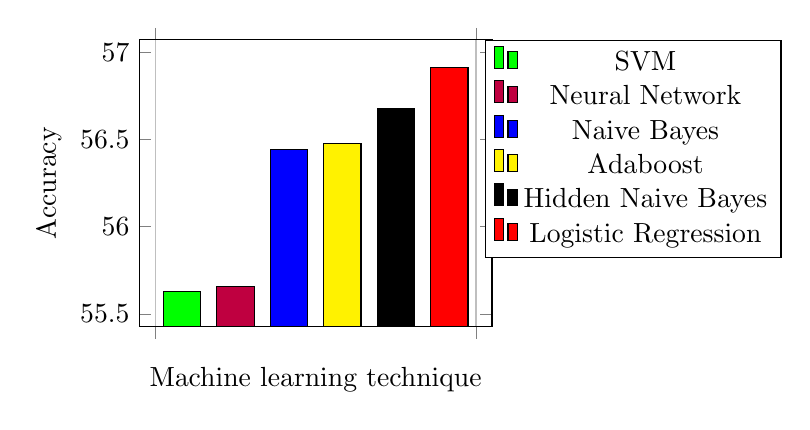
\begin{tikzpicture}
    \begin{axis}[
      %x tick label style={/pgf/number format/1000 sep=},
      xticklabel=\empty,
      ylabel=Accuracy,
      xlabel=Machine learning technique,
      enlargelimits=0.05,
      legend style={at={(1.4,1.0)},
        anchor=north,legend columns=1},
      ybar interval=0.7,
      width=.50\textwidth,
      ymin=55.5, ymax=57,
      reverse legend,
      ]
      \addplot[fill=red] coordinates {(1,56.916) 
        (0,2)
      };
      \addplot[fill=black] coordinates {(1,56.6807) 
        (0,56.6807)
      };
      \addplot[fill=yellow] coordinates {(1,56.479) 
        (0,2)
      };
      \addplot[fill=blue] coordinates {(1,56.4454) 
        (0,56.4454)
      };
      \addplot[fill=purple] coordinates {(1,55.6555) 
        (0,0)
      };
      \addplot[fill=green] coordinates {(1,55.63)
        (0,0)
      };
      \legend{Logistic Regression,Hidden Naive Bayes,Adaboost,Naive Bayes,Neural Network,SVM}
    \end{axis} 
  \end{tikzpicture}
  \caption{Test of best machine learning technique}\label{fig:besttech}
\end{figure}



\subsubsection{Implementation comparison}
To test if Apache Sparks PySpark implementation of logistic regression is implemented properly, it is compared to the equivalent implementations in Weka and R. The data consists of 5000 matches where Weka uses a sparse presentation, while R uses a dense and PySpark the raw file with JSON elements. As seen in \Cref{tab:impl_results}, the implementations are close to equal, the minor differences could be caused by differences in the parameter settings. However these results confirm that all implementations are acceptable and further testing can be performed in any of the environments.

\begin{table}[!htb]
  \centering
  \begin{tabular}{|l|c|}
    \hline
    Implementation  & Accuracy  \\
    \hline
    Weka & 55\%  \\
    R & 55\%\\
    PySpark & 53\%\\ 
    \hline
  \end{tabular}
  \caption{Implementation comparison results}
  \label{tab:impl_results}
\end{table}

\subsubsection{Feature representation test}
Features can be presented in many different ways and this test is constructed to finding the best way to that. The representations that will be tested are the methods presented in \Cref{sec:representationoffeatures}. The test was done on an increasing number of matches with all the different methods to check how they hold up with much data. As the result, shown in \Cref{fig:feat-rep}, indicates, method 1 and 4 are very close, but binary being slightly above ternary majority of the time, which is the reason for us choosing binary.

\begin{figure}[!htb]
  \centering
  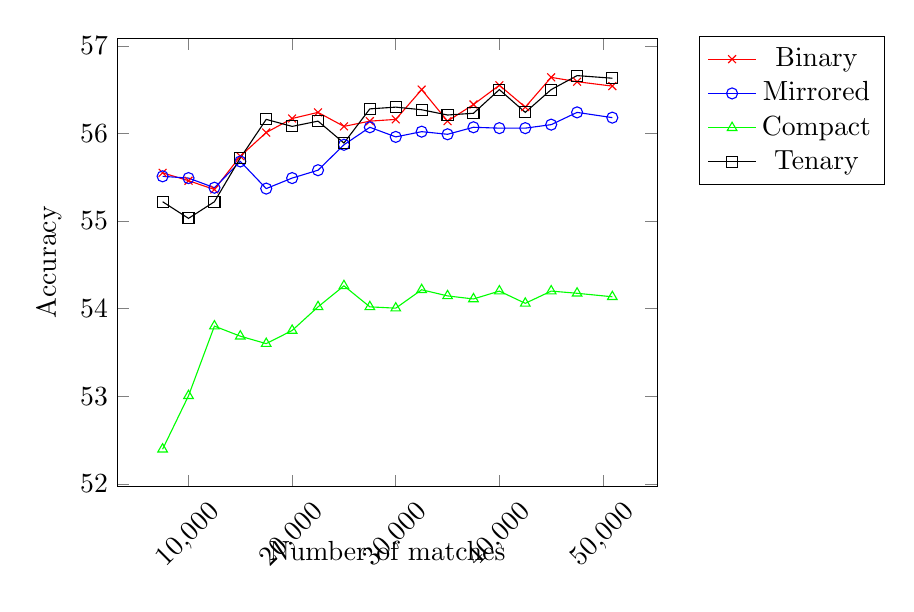
\begin{tikzpicture}[] 
    \begin{axis}[
      xlabel=Number of matches, 
      ylabel=Accuracy,
      xtick={10000,20000,30000,40000,50000},
      xticklabel style={rotate=45,anchor=near xticklabel},
      scaled x ticks=false,
      x label style={at={(axis description cs:0.5,-0.1)},anchor=north},
      legend style={at={(1.25,1.005)},
        anchor=north,legend columns=1},] 
      \addplot[color=red,mark=x] coordinates { 
        (7500, 55.55)
        (10000, 55.46)
        (12500, 55.36)
        (15000, 55.74)
        (17500, 56.01)
        (20000, 56.17)
        (22500, 56.24)
        (25000, 56.08)
        (27500, 56.14)
        (30000, 56.16)
        (32500, 56.50)
        (35000, 56.14)
        (37500, 56.33)
        (40000, 56.55)
        (42500, 56.30)
        (45000, 56.64)
        (47500, 56.59)
        (50901, 56.54)
      };
      \addplot[color=blue,mark=o] coordinates { 
        (7500, 55.51)  
        (10000, 55.49)
        (12500, 55.38)
        (15000, 55.68)
        (17500, 55.37)
        (20000, 55.49)
        (22500, 55.58)
        (25000, 55.87)
        (27500, 56.07)
        (30000, 55.96)
        (32500, 56.02)
        (35000, 55.99)
        (37500, 56.07)
        (40000, 56.06)
        (42500, 56.06)
        (45000, 56.10)
        (47500, 56.24)
        (50901, 56.18)
      };
      \addplot[color=green,mark=triangle] coordinates { 
        (7500, 52.395)  
        (10000, 53.005)
        (12500, 53.80)
        (15000, 53.685)
        (17500, 53.60)
        (20000, 53.75)
        (22500, 54.02)
        (25000, 54.26)
        (27500, 54.02)
        (30000, 54.005)
        (32500, 54.215)
        (35000, 54.145)
        (37500, 54.11)
        (40000, 54.20)
        (42500, 54.06)
        (45000, 54.20)
        (47500, 54.175)
        (50901, 54.135)
      };
      \addplot[color=black,mark=square] coordinates {
        (7500, 55.22)  
        (10000, 55.03)
        (12500, 55.22)
        (15000, 55.72)
        (17500, 56.16)
        (20000, 56.08)
        (22500, 56.14)
        (25000, 55.89)
        (27500, 56.28)
        (30000, 56.30)
        (32500, 56.27)
        (35000, 56.21)
        (37500, 56.23)        
        (40000, 56.50)
        (42500, 56.24)
        (45000, 56.50)
        (47500, 56.66)
        (50901, 56.63)
      };
      \legend{Binary, Mirrored, Compact, Tenary}
    \end{axis} 
  \end{tikzpicture}
  \caption{Test for representation of features}\label{fig:feat-rep}
\end{figure}

\subsubsection{Feature tests}\label{sec:feattest}
Some features might be more expressive than others, and finding the set of features that will yield the best result is imperative. The test on the cluster is performed with logistic regression using stochastic gradient descent and L2 regularization with a ridge value of 0.01. 
For each feature test 1348428 games is used for training and 577552 games are used for evaluation. 
The feature sets tested are:
\begin{itemize}
\item blue team, red team 
\item blue combos, red combos
\item blue team, red team, blue combos, red combos
\item blue team, red team, blue combos, red combos, cross team combos
\item blue team, red team, blue combos, red combos, cross team combos, champion ranks
\item all pregame features 
\end{itemize}

For each set of features the total possibilities of features is given, as well as the amount of features extracted from a single game. Along with the numbers is given a reasoning for testing the features.  
\\\\
\textbf{Blue team, red team} \\
As mentioned in each team picks 5 champions, from a pool of 124 champions, depending on the game mode this results in a total of 248 or 243 features, of which 10 is picked. The feature representation is chosen since it is the simples features we have representing a game. \\\\
\textbf{Blue combos, red combos} \\
As mentioned in there might be some synergy between combinations of champions. The total number combos for each team is calculated as $n \times (n-1)/2$. Depending on the game mode the total amount of features is calculated as:  
\begin{itemize}
\item $124 \times (124-1)/2 + 124 \times (124-1)/2 = 15252$
\item $124 \times (124-1)/2 + 119 \times (119-1)/2 = 14647$
\end{itemize}
From the possible features $20$ is represented for each match. \\\\
\textbf{Blue team, red team, blue combos, red combos} \\
This feature test is added to test how well the extension from team to combos works with the individual players. The total features again depends on the game mode and is either: 
\begin{itemize}
\item $248 + 15252 = 15500$
\item $243 + 14647 = 14890$
\end{itemize}
The total features pick for each game is 30.\\\\
\textbf{Blue team, red team, blue combos, red combos, cross team combos}\\
The cross team combos is calculated as mentioned in, the reasoning behind this feature is that some champions might have special skills which counters the skills on another champion. 
Depending on the game mode the total amount of features for cross team combos is: 
\begin{itemize}
\item $15500+124\times124 = 30876$
\item $14890+119\times119 = 29051$
\end{itemize}
From this pool of features 80 is represented in each match.\\\\
\textbf{Blue team, red team, blue combos, red combos, cross team combos, champion ranks}\\
For each player their best achieved rank in the previous season is known there are 8 possible ranks. The total features for this test is: 
\begin{itemize}
\item $30876 + 248\times8 = 32860$
\item $29051 + 248\times8 = 31035$
\end{itemize}
From this pool of features 90 is represented in each match. \\\\
\textbf{All pre-match features}\\
All pre-match features is a combination of, blue team, red team, blue combos, red combos, cross team combos, champion ranks, champions lanes, best team rank, champion queue type, champion runes, champion masteries and champion spell combo.  

Champion lanes describe which lane a given champion is played on e.g. a champion might perform better if played in the middle lane instead of the top lane. Best team rank is a measure of how skilled the two teams are. Champion queue type combines the champion picked by a player with the game mode being played. Champion runes combines the champion picked with the runes of the player who picked the champion (runes are used to boot certain skills of a champion, e.g. give a champion higher starting health).
\begin{figure}[!htb]
  \centering
  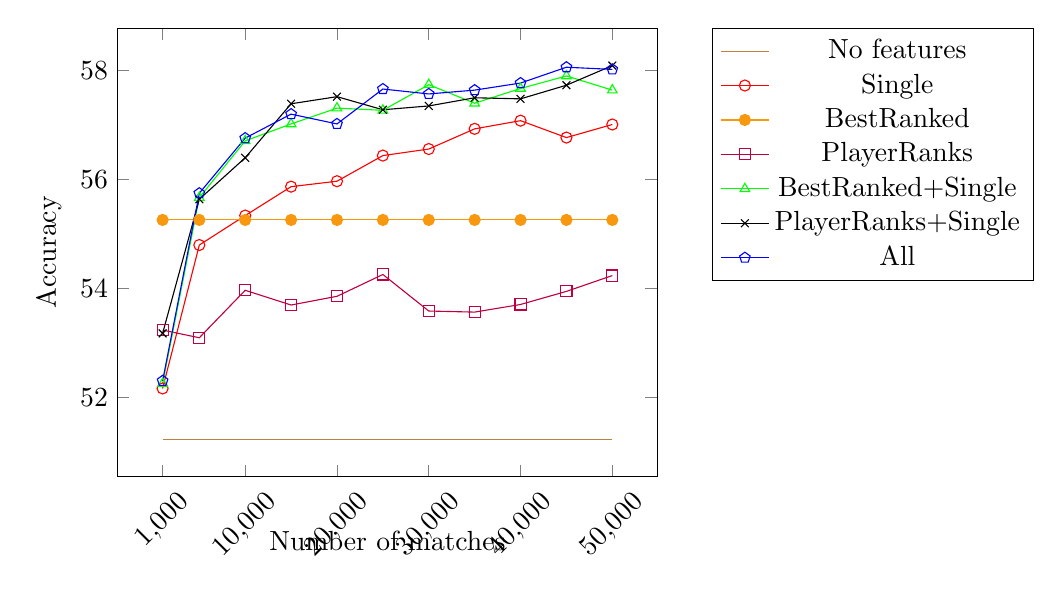
\begin{tikzpicture}[] 
    \begin{axis}[
      xlabel=Number of matches, 
      ylabel=Accuracy,
      xtick={1000,10000,20000,30000,40000,50000},
      xticklabel style={rotate=45,anchor=near xticklabel},
      scaled x ticks=false,
      x label style={at={(axis description cs:0.5,-0.1)},anchor=north},
      legend style={at={(1.4,1.001)},
        anchor=north,legend columns=1},] 
      \addplot[color=brown] coordinates { 
        (1000,51.24)
        (5000,51.24)
        (10000,51.24)
        (15000,51.24)
        (20000,51.24)
        (25000,51.24)
        (30000,51.24)
        (35000,51.24)
        (40000,51.24)
        (45000,51.24)
        (50000,51.24)
      };
      \addplot[color=red,mark=o] coordinates { 
        (1000,52.17)
        (5000,54.8)
        (10000,55.34)
        (15000,55.87)
        (20000,55.97)
        (25000,56.44)
        (30000,56.56)
        (35000,56.93)
        (40000,57.08)
        (45000,56.77)
        (50000,57.01)
      };
      \addplot[color=YellowOrange,mark=*] coordinates { 
        (1000,55.26)
        (5000,55.26)
        (10000,55.26)
        (15000,55.26)
        (20000,55.26)
        (25000,55.26)
        (30000,55.26)
        (35000,55.26)
        (40000,55.26)
        (45000,55.26)
        (50000,55.26)
      };
      \addplot[color=purple,mark=square] coordinates { 
        (1000,53.24)
        (5000,53.1)
        (10000,53.97)
        (15000,53.7)
        (20000,53.86)
        (25000,54.26)
        (30000,53.59)
        (35000,53.57)
        (40000,53.71)
        (45000,53.95)
        (50000,54.24)
      };
      \addplot[color=green,mark=triangle] coordinates { 
        (1000,52.26)
        (5000,55.67)
        (10000,56.71)
        (15000,57.02)
        (20000,57.31)
        (25000,57.27)
        (30000,57.74)
        (35000,57.4)
        (40000,57.67)
        (45000,57.9)
        (50000,57.64)
      };
      \addplot[color=black,mark=x] coordinates { 
        (1000,53.18)
        (5000,55.64)
        (10000,56.4)
        (15000,57.39)
        (20000,57.52)
        (25000,57.28)
        (30000,57.35)
        (35000,57.5)
        (40000,57.48)
        (45000,57.73)
        (50000,58.09)
      };
      \addplot[color=blue,mark=pentagon] coordinates { 
        (1000,52.31)
        (5000,55.75)
        (10000,56.76)
        (15000,57.2)
        (20000,57.02)
        (25000,57.66)
        (30000,57.57)
        (35000,57.64)
        (40000,57.77)
        (45000,58.06)
        (50000,58.02)
      };
      \legend{No features,Single,BestRanked,PlayerRanks,BestRanked+Single,PlayerRanks+Single,All}
    \end{axis} 
  \end{tikzpicture}
  \caption{Accuracy of features}\label{fig:best-feat}
\end{figure}

\subsection{Cluster tests}\label{sec:clustertest}
In this section the tests that requires the cluster. This is due to the size of the tests, and the expected time frame.
\subsubsection{Big data improvements}
To test if big data gives an improvement when predicting the outcome of a match, the same features and method where used on an increasing sized data starting from 1000 matches. After the model was made, it was tested on the training data, as a $\frac{2}{3}$-split and finally cross-validation. And as seen on \Cref{fig:bigdata} there will be more information once more tests has been run!

\begin{figure}[!htb]
  \centering
  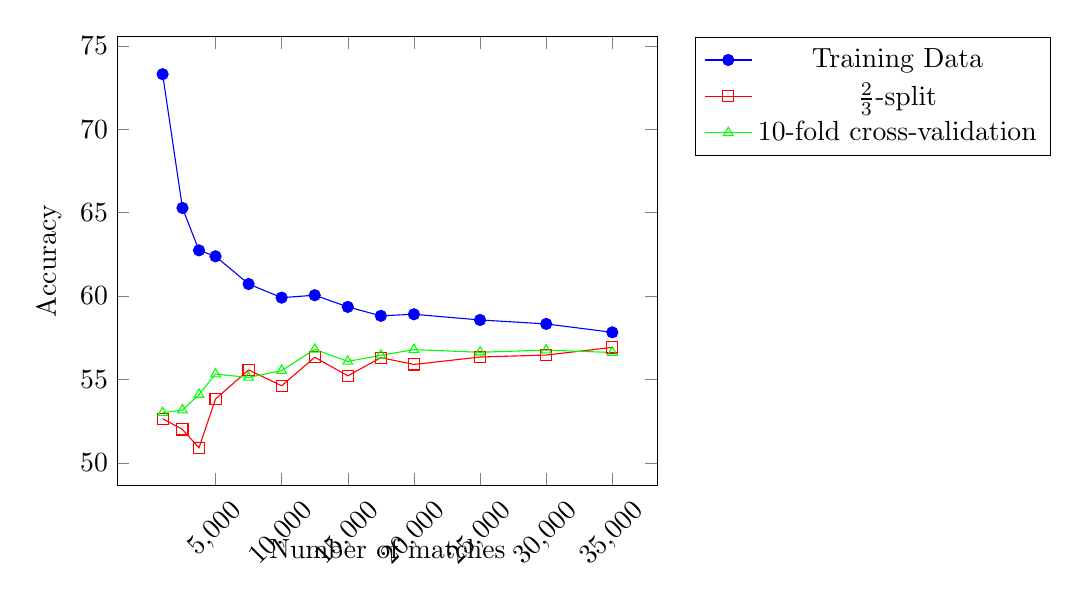
\begin{tikzpicture}[] 
    \begin{axis}[
      xlabel=Number of matches, 
      ylabel=Accuracy,
      xtick={5000,10000,15000,20000,25000,30000,35000},
      xticklabel style={rotate=45,anchor=near xticklabel},
      scaled x ticks=false,
      x label style={at={(axis description cs:0.5,-0.1)},anchor=north},
      legend style={at={(1.4,1.0)},
        anchor=north,legend columns=1},] 
      \addplot[color=blue,mark=*] coordinates {
        (1000, 73.3)   	
        (2500,65.28)  	
        (3750,62.7367)	
        (5000,62.38)
        (7500,60.72)
        (10000,59.9)
        (12500,60.048)
        (15000,59.3467)
        (17500,58.8114)
        (20000,58.905)
        (25000,58.564)
        (30000,58.3267)
        (35000,57.8229)
      };
      \addplot[color=red,mark=square] coordinates {
        (1000,52.6471)
        (2500,52)
        (3750,50.902)
        (5000,53.8235)
        (7500,55.5686)
        (10000,54.6176)
        (12500,56.3294)
        (15000,55.2157)
        (17500,56.3025)
        (20000,55.8971)
        (25000,56.3412)
        (30000,56.4608)
        (35000,56.916)
      };
      \addplot[color=green,mark=triangle] coordinates {
        (1000,53)
        (2500,53.16)
        (3750,54.0944)
        (5000,55.32)
        (7500,55.12)
        (10000,55.53)
        (12500,56.8)
        (15000,56.08)
        (17500,56.4457)
        (20000,56.785)
        (25000,56.628)
        (30000,56.7567)
        (35000,56.6143)
      };
      \legend{Training Data, $\frac{2}{3}$-split, 10-fold cross-validation}
    \end{axis} 
  \end{tikzpicture}
  \caption{Test for representation of features}\label{fig:bigdata}
\end{figure}

\subsubsection{Speed up}
This test is constructed to show that an increasing number of nodes increases the computation speed. As seen in \Cref{sec:clustersetup}, the cluster consists of 4 nodes, this means the test will be run with the master and either 1, 2 or 3 nodes. The data for this test be the same to make the results comparable.

\begin{table}[!htb]
  \centering
  \begin{tabular}{|c|c|}
    \hline
    Number of nodes & Time taken\\
    \hline
    1 & ? \\
    2 & ? \\
    3 & ? \\
    \hline
  \end{tabular}
  \caption{Speed up test results}\label{tab:speedup}
\end{table}

\subsubsection{Prediction with team ranks}
Previous seasons rank for each player is registered in the match data. This test is constructed to test whether this rank alone is a useful feature when predicting a winning team.
\subsubsection{Prediction with all features}
All the features created from the data is used for this test. 
\subsubsection{Prediction with all features except lane}
This test is almost identical to the test seen above, except the lane feature is excluded. This test is performed to learn if the lane each hero choses to defend influences the outcome of the match and if this is actually useful when predicting outcome of future matches.
\subsubsection{Prediction using support vector machine}
The above tests will for this test be performed using support vector machine to see how it compares to logistic regression. 
\subsubsection{Prediction with best features}
The test for prediction with best features will use the features that were determined as the best in \Cref{sec:feattest}. This is done to see how well the prediction can be made at all. This should, should we play the game, give us the opportunity to pick champions that counter those of the opponents team, thus increasing our chances of winning.
\subsubsection{Sample size}
Text.


%%% Local Variables:
%%% mode: latex
%%% TeX-master: "../main"
%%% End:


\section{Conclusion}

\bibliography{Literature}



% APPENDIX
\newpage
\appendix
\section{Setting up the Cluster}
\label{sec:hadoop}
To set up a cluster with equal settings to ours, all the machines must be running Debian Wheezy 7.0 32-bit (linux) and connected via switch with static ip. In addiction, one machine must be chosen as the master and the following packages must be installed on all machines:
\begin{itemize}
\item openssh 
\item openssh-server 
\item openjdk-7-jre 
\item openjdk-7-jdk 
\end{itemize}
Now create a new user for the cluster setup, this is considered good practice. The \emph{username} must be the same name across all machines.
\lstset{language=bash}
\begin{lstlisting}
  adduser ``username''
\end{lstlisting} %Maybe rethink quotes in the listing
To easier work with the IP's of the machines, set up a file called \emph{hosts}:
\begin{verbatim}
127.0.0.1 localhost

ip node1
ip node2
ip node3
...
\end{verbatim}
Which is saved in the hosts directory: 
\begin{verbatim}
/etc/hosts
\end{verbatim}
Following that, each machine needs ssh configured, where \emph{node-id} is the alias created in the \emph{hosts} file. Run the following commands in the terminal of each master to each slave and from each slave to master:
\begin{lstlisting}
  ssh-keygen
  ssh-copy-id ``username@node-id''
\end{lstlisting}

\subsection{Setting up Hadoop}
All of the following steps must be done on all machines. To set up Hadoop, create a hadoop group, then add the users previously created to that group:
\begin{lstlisting}
  addgroup hadoop
  adduser ``username'' hadoop
\end{lstlisting}
At this point Hadoop 2.6.0 32-bit should be downloaded and installed in the path \textsf{/usr/local/hadoop}. We then change the owner of the hadoop directory so we have the correct access:
\begin{lstlisting}
  chown -R username:username /usr/local/hadoop
\end{lstlisting}
The following will be put in \emph{/home/username/.bashrc} file:
\begin{verbatim}
export JAVA_HOME=/usr/lib/jvm/java-7-openjdk-i386
export HADOOP_INSTALL=/usr/local/hadoop
export PATH=$PATH:$HADOOP_INSTALL/bin
export PATH=$PATH:$HADOOP_INSTALL/sbin
export HADOOP_MAPRED_HOME=$HADOOP_INSTALL
export HADOOP_COMMON_HOME=$HADOOP_INSTALL
export HADOOP_HDFS_HOME=$HADOOP_INSTALL
export YARN_HOME=$HADOOP_INSTALL
\end{verbatim}
In the file \emph{hadoop-env.sh} found in \textsf{/usr/local/hadoop/etc/hadoop/} the line \emph{JAVA\_HOME} should be replaced with \emph{export JAVA\_HOME=/usr/lib/java-7-openjdk-i386}.
In addition the \emph{core-site.xml} which is found in \textsf{/usr/local/hadoop/etc/hadoop/} needs an added property inside the configuration tag: 
\begin{verbatim}
<property>
  <name>fs.defaultFS</name>
  <value>hdfs://MASTER:9000</value>
</property>
\end{verbatim}
\emph{MASTER} needs to be replaced with the hostname for the master node. Another file that needs added properties is \emph{hdfs-site.xml}, which can be found in the folder \textsf{/usr/local/hadoop/etc/hadoop/}:
\begin{verbatim}
<property>
  <name>dfs.namenode.data.dir</name>
  <value>file:/home/username/data/hdfs/namenode</value>
</property>

<property>
  <name>dfs.datanode.data.dir</name>
  <value>file:/home/username/data/hdfs/datanode</value>
</property>
\end{verbatim}
These should also be added in the configuration tag.
The final thing that needs for Hadoop to run is for the master to know the slaves. Create a file called \emph{slaves} in \textsf{/usr/local/hadoop/etc/hadoop/} with all the hostnames of slaves listed separated by newline:
\begin{verbatim}
node1
node2
...
\end{verbatim}

\subsection{Setting up Apache Spark}
All of the following steps must done on all machines. To get Spark 1.2.1 running, download the hadoop 32-bit precompiled version and install it to \textsf{/usr/local/spark} and again run the command to set up the correct rights:
\begin{lstlisting}
  chown -R username:username/usr/local/spark
\end{lstlisting}
The final step for setting up Apache Spark is copying the previous \emph{slaves} file into the folder \textsf{/usr/local/spark/conf/}.

\subsection{Starting the cluster}
To start the cluster the master has to run the following commands:
\begin{lstlisting}
  start-dfs.sh
  cd /usr/local/spark
  ./sbin/start-all.sh
\end{lstlisting}
Now the cluster is ready to use.

\subsection{Adding files}
To add files to the file system use the following script:
\begin{lstlisting}
  string = $(hdfs dfs -ls hdfs://node1:9000/)
  for file in "file path"*
  do
  name = $(file##*/)

  if [[$string == *$name* ]]
  then
    echo 'file exists'
  else
    hdfs dfs -copyFromLocal $file hdfs://node1:9000/$name
    echo 'adding new file'
  fi 

  done
\end{lstlisting}
This will add all the files, that does not already exist, from the given folder to the hdfs file system.


%%% Local Variables:
%%% mode: latex
%%% TeX-master: "../main"
%%% End:

\begin{frame}{Finding the Best Model}

% run on a single machine
Tested Classifiers

\begin{itemize}
\item Naive Bayes 
\item Logistic Regression
\item Neural Network
\item Support Vector Machine
\item Adaboost
\item Hoeffding tree
\item Decision Stump
\end{itemize}
%\vspace{20cm}
\end{frame}

\begin{frame}{Finding the Best Model}
\begin{itemize}
\item Data \begin{itemize}
		\item 2/3 Training
		\item 1/3 Testing
           \end{itemize}
\item Parameters? 

\end{itemize}

\end{frame}

\begin{frame}{Finding the Best Model}

\begin{figure}[!htb]
\centering
  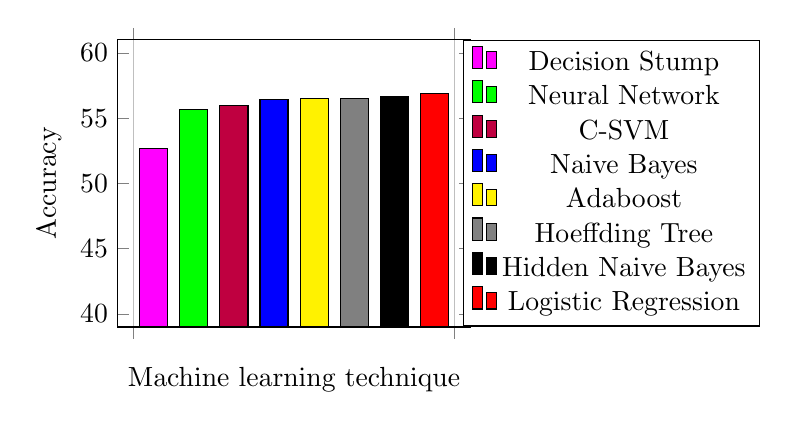
\begin{tikzpicture}
    \begin{axis}[
      %x tick label style={/pgf/number format/1000 sep=},
      xticklabel=\empty,
      ylabel=Accuracy,
      xlabel=Machine learning technique,
      enlargelimits=0.05,
      legend style={at={(1.4,1.0)},
        anchor=north,legend columns=1},
      ybar interval=0.7,
      width=.50\textwidth,
      ymin=40, ymax=60,
      reverse legend,
      ]
      \addplot[fill=red] coordinates {(1,56.916) 
        (0,2)
      };
      \addplot[fill=black] coordinates {(1,56.6807) 
        (0,56.6807)
      };

\addplot[fill=gray] coordinates {(1,56.48)
        (0,0)
      };      
            
      \addplot[fill=yellow] coordinates {(1,56.479) 
        (0,2)
      };
      \addplot[fill=blue] coordinates {(1,56.4454) 
        (0,56.4454)
      };
      \addplot[fill=purple] coordinates {(1,55.98)
        (0,0)
      };
      \addplot[fill=green] coordinates {(1,55.6555) 
        (0,0)
      };      
      \addplot[fill=Fuchsia] coordinates {(1,52.64)
        (0,0)
      };
      \legend{Logistic Regression,Hidden Naive Bayes,Hoeffding Tree,Adaboost,Naive Bayes,C-SVM,Neural Network, Decision Stump}
    \end{axis} 
  \end{tikzpicture}
%  \caption{ue}\label{fig:besttech}
\end{figure}

\end{frame}

\begin{frame}{Logistic Regression}

\[ L_D(\textbf{w}) = \sum_{n=1}^N (y_n-\hat{y}_n)^2 = \sum_{n=1}^N \left(y_n - \sum_{i=0}^M w_i \phi_i(x_n)\right)^{2} \] 

\end{frame}

\begin{frame}{Logistic Regression}

\[ \hat{y} = \sigma(h_w(x)) = \frac{1}{1+e^{-h_w(x)}} \]

\[E_w(y,h_w(x)) = \begin{cases}
	-ln(\sigma(h_w(x))) &\text{if y = 1}\\	
	-ln(1-\sigma(h_w(x))) &\text{if y = 0}
\end{cases}\]

\end{frame}

\begin{frame}{Regularisation}

\[ L(\mathbf{w})
  = L_D(\mathbf{w}) + L_w 
  = \sum_{n=1}^N E_w(y_n, h_w(x_n)) + \frac{\lambda}{2} \sum_{m=1}^{M} {w_m}^2 \] 

\end{frame}

\begin{frame}{Stochastic Gradient Descent}

\[ w_j^{(i)} = w_j^{(i-1)} - \eta \frac{\partial E_{w^{(i-1)}}(y_n, h_{w^{(i-1)}}(x_n))}{\partial w_j^{(i-1)}} \]

\end{frame}


\begin{frame}{Simulated Annealing}

$$\eta_i = \frac{1}{(1+i)^\alpha}$$


With an $\alpha$ chosen in the interval $(0.5,1]$. 

\end{frame}


%\begin{frame}
%\end{frame}



\section{Data and Feature Setup}\label{sec:features}
In \Cref{sec:matchdata} we investigate the match data made available by the Riot's API, which covers almost any detail of a match.
\Cref{sec:choosingfeatures} identifies a number of features that can be extracted from match data, which we think are most important when it comes to prediction of the winning team. The choice is based on our intuition as more or less experienced LoL players. The size of each type of features domain is calculated in \Cref{sec:featuresparsity}, as well as the sparsity with regards to how many features that appear in each match.
In \Cref{sec:representationoffeatures}, a possible feature symmetry issue is investigated which raises a number of concerns and suggestions for solutions as to how the extracted features should be represented. 


\subsection{League of Legends Match Information}\label{sec:matchdata}
Riot records large amounts of information about played matches and players~\cite{matchinfo}. Much, if not all, of this data is publicly available through their online API. In this paper the focus will be on the match data only, and more particularly the data that can be extracted before a match starts. The only exception is information about which team that won each match. Since we want to predict who wins, we need that data to train and evaluate a classifier.
We have chosen to extract the following data from each match:
\begin{itemize}
\item Winning team
\item Champions on each of the two teams
\item The rank of all players
\item Game mode
\item Queue type
\end{itemize}
And the following data from each player:
\begin{itemize}
\item Lane occupied 
\item Runes 
\item Masteries 
\item Summoner spells 
\end{itemize}
All the extracted information has be chosen because we think it might be useful for estimating how good a particular team is against another team. \todo{kommetar: dårlig begrundelse}
The champions on each of the two teams have been included because some champions may be better than others.
The rank of players are considered because the rank system in LoL aims to assign better players a greater rank. Intuitively, a team of high ranked players must be better than a team of low ranked players.
The lane played by each player may be useful, because players often stick to one particular lane for the first half a match.
Note that the lanes of the opponent team is not known before the game starts, but we have still chosen to include it, because it very often can determined based on the picked champions. Knowing the lane of the players means knowing the ranks and champion of the players that most often fights against each other.
Both the masteries, runes. and summoner spells are worth knowing, because each of them add or improve some property of a champion. 
%The summoner spells are also worth considering because they adds additional properties to a champion.
Different game modes imply different play styles. By only considering the 5 versus 5 game mode, we hope to achieve better predictions.
The queue type of the match lets us know if the LoL match making system has formed the two teams, or the players have formed the two teams themselves.
Teams formed on their own may be better, because the players in self formed teams often know each other better and more often use voice communication tools.
Finally the matches patch version is used to make sure that we only use matches from the same patches. Different patches may change aspects of the game, e.g.\ the strength of particular champions, and without accounting for different patches, the trained classifier accuracy may decrease.  

The data set we use use consists of matches played from $23^{\text{rd}}$ of March 2015 to $27^{\text{th}}$ of March 2015. It includes match details for matches played across the world. When filtering the games to include only 5 versus 5 game modes, we are left with 1925980 matches. The patch version of all matches used is $5.6$.


%%% Local Variables:
%%% mode: latex
%%% TeX-master: "../main"
%%% End:


\end{document}

%%% Local Variables:
%%% mode: latex
%%% TeX-master: t
%%% End:
